\section{Framework and overview}\label{sec:framework}

\begin{figure}[h]
\centering
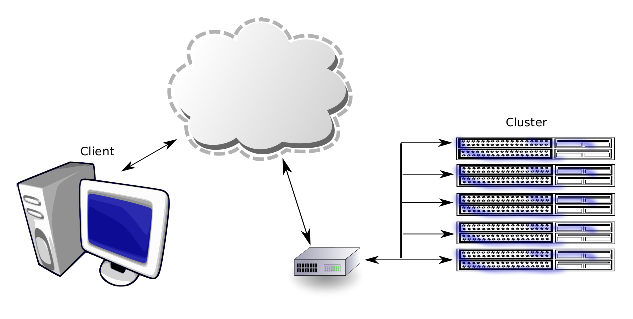
\includegraphics[scale=0.85]{img/framework.eps}
\caption{Testbed setting used for evaluation}
\label{fig:framework}
\end{figure}

\subsection{testbed}
Our testbed consists of a cluster of five machines connected by a switch. These nodes will be the servers hosting Zookepper instances. Another machine, we will call it the client machine, will act as the user of Zookeeper. The Round-Trip Time~(RTT) between machines in the cluster is around 0.1ms and around 0.2ms for client to cluster communication. Each cluster machine has a 5 quad-core Xeon \note{type and clock} with commodity 500GB 7.2k rpm disks. They are interconnected with a single 1Gbps Ethernet switch.

\subsection{consensus protocol}
It is important for distributed systems to have a well-defined consensus protocol. High latency and possibility of failures make achieving consensus an intricate task. For this matter consensus protocols such as Two-Phase Commit~(2PC), Three-Phase Commit~(3PC), and paxos were proposed. In this section we will focus on paxos due its use in distributed consensus servres, such as Chubby and, to some degree, Zookeeper. The use of paxos over other alternatives is its resilience to node and network failures. In addition, paxos does not need a fail recovery model.

At each iteration, a \emph{proposer} initiates the protocol and send a proposal to other nodes. Each proposal is tagged with a unique sequence number. Other nodes are called \emph{acceptors}. When acceptors receive proposals, they would either accept or reject. Accepting a proposal is essentially a promise not to accept other proposals with lower sequence numbers. When a majority (quorum) of servers accept a value, then the proposer can proceed with committing the proposal by sending a commit message to all followers. 

\subsection{Zookeeper}
Zookeeper is an open-source coordination service for distributed systems. It runs as a set of replicated distributed servers. A leader election mechanism is used. All requests are forwarded to the leader. A consensus protocol is used to agree on received requests. A combined transaction and write-ahead logging is used in a variant of Paxos as a consensus protocol. Zookeeper levarage an \emph{atomic broadcast} protocol in their consensus protocol implementation. Clients can connect to any of those replicas and issue operations. Zookeeper maintains an order of operations. Each update is stamped. This stamp can then be levaraged in higher level abstractions. Guarantees made by Zookeeper to clients' operations include the following:
\begin{itemize}
\item{\emph{Sequential consistency}: operations are executed in the order they were received. }
\item{\emph{Atomicity}: operations are either completely executed or aborted. }
\item{\emph{Single system image}: all servers maintain the same view. }
\item{\emph{Reliability}: updates are persistent. }
\item{\emph{Timeliness}: updates will be reflected on all servers within a specified time bound. }
\end{itemize}
These guarantees will aid us in reasoning on the way we use Zookeeper operations. The set of offered operations enable more complex services such as coordination, synchronization, configuration management, and naming. These operations operate on a Unix-like filesystem tree architecture. Each file has a path and could be either \emph{permanent} or \emph{ephemeral}. Permenant files persist a client's disconnection whereas ephemeral files are deleted when a client disconnects. Those "files" are called \emph{znodes}. A useful zookeeper primitive is \emph{watch}. A user can set a watch on a znode. When a change on the state of that znode occur, the watch is triggered and the user is informed on the new state of the znode. We now summarize Zookeeper operations of our interest:
\begin{itemize}
\item{\emph{create}: create a znode by specifying a path. A \emph{sequenced} flag can be used to tell Zookeeper to append the znode name with a monotonically increasing identifier. Pathname is returned if create is successful. Otherwise, an exception is returned.}
\item{\emph{delete}: deletes a znode.}
\item{\emph{exists}: checks if a znode exists on a supplied location.}
\item{\emph{getChildren}: return a list of children of a znode, hence files in a folder.}
\end{itemize}
Each one of those operations have two implementations, a synchronous and an asynchronous ones. Synchronous operations block until a reply is received from the server. On the other hand, asynchronous operations returns immediately and a callback is set on the client side to receive from the server when operation is complete.

\begin{figure}[h]
\centering
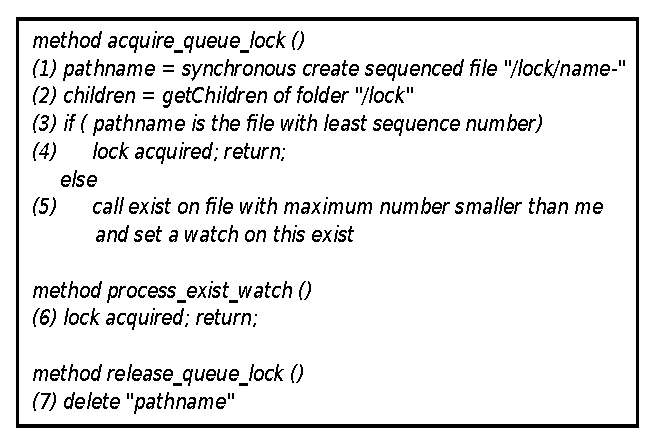
\includegraphics[scale=0.85]{img/queue_lock_pseudo.eps}
\caption{Pseudo code of acquiring and releasing queue locks}
\label{fig:queue_lock_pseudo}
\end{figure}

\begin{figure}[h]
\centering
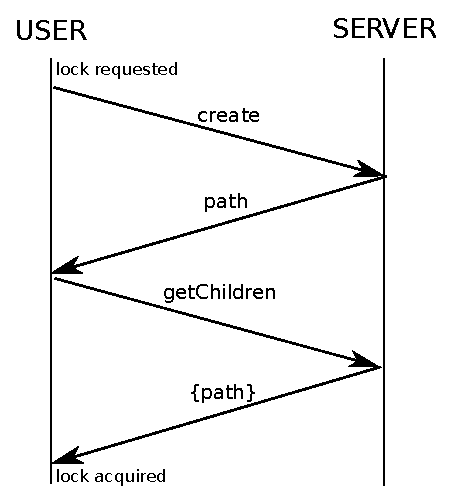
\includegraphics[scale=0.85]{img/queue_lock_time.eps}
\caption{A time diagram showing time required to acquire a queue lock if no other user is holding it}
\label{fig:queue_lock_time}
\end{figure}

\begin{figure}[h]
\centering
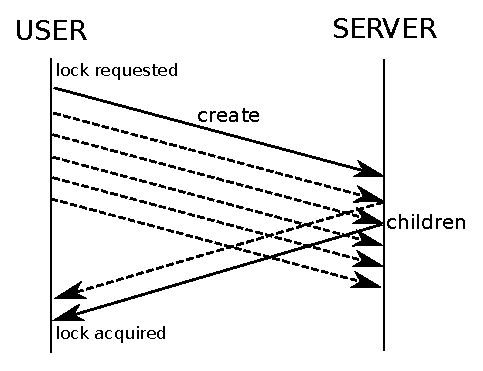
\includegraphics[scale=0.85]{img/async_queue_lock_time.eps}
\caption{A time diagram showing time required to acquire a queue lock if no other user is holding it using asynchronous calls. Dashed arrows from user to server are getChildren operations. Dashed arrows from server to user represent getChildren replies before the lock is acquired. Solid arrow from server to user is getChildren reply with user having the smallest sequenced file. The callback for asynchronous create is not shown.}
\label{fig:async_queue_lock_time}
\end{figure}

\subsection{synchronization primitives}

One of the main points studied in this paper is the effectiveness of synchronization primitives (primitives) and their comparative behavior giving different network conditions. Here we give a summary of the primitives we consider. Primitives are queue locks and test-and-set~(TAS). We divide primitives to synchronous and asynchronous depending on the client-server interactions. In the following we will summarize those primitives and how they translate in distributed systems using Zookeeper operations:
\begin{itemize}
\item{Synchronous queue lock: a queue structure maintaing the process of acquiring a lock. If a user tried to acquire a lock while another was holding it, then it is queued. Thus, users acquire the lock based on the order in which they entered the queue, helping achieve fairness. This is implemented in Zookeeper by synchronously creating an ephemeral, sequenced znode. Each create operation will return the file name, indicating the sequence number. The client waits until it has the smallest sequence number. Then, it acquire the lock. Releasing the lock is done by merely deleting the corresponding file. Pseudo code is displayed in Figure~\ref{fig:queue_lock_pseudo}. There are two possible execution paths. First, a user tries to acquire a lock while no one is holding it. In this case algorithm exist in line (4) after calling only two Zookeeper operations, namely synchronous \emph{create} and \emph{getChildren}. Second, another user is holding the lock when we try to acquire it. In this case the total latency is of operations \emph{creat}, \emph{getChildren}, and \emph{exists}, in addition to waiting time until the \emph{watch} returns to the client.}
\item{Synchronous TAS: to acquire a lock, the user repeatedly execute TAS until it succeeds. TAS tests a boolean flag until it flips it from false to true. Traditionally, TAS surfaced in memory-sharing systems due to the advent of atomic TAS operations. In Zookeeper we are able to create a primitive that is similar in spirit to hardware TAS. A user tries to create a file with a known name (all users try to create the same file). If the file already existed that means that another user is holding the lock and create will return an exception. Otherwise, the user will hold the lock. To release the lock, the user deletes the file. We repeatedly try to acquire a lock by calling \emph{create} in a busy loop. Alternatively, a watch on the file can be used to avoid busy waiting. Apparently, there is no order in entering the queue, hurting fairness. Execution path of TAS when no user is holding the lock is only one synchronous \emph{create} call. Otherwise, it is the time until the user is the fastest to create the file. A more detailed analysis of wait times are found in the analysis section. }
\item{Asynchronous primitives: We showed synchronous implementations of our primitives. In them, we use synchronous versions of Zookeeper operations. Thus, we block until we receive a reply from the server. It is found, however, that we can cut some latency by using asynchronous operations and continuously poll servers for desired state. For example, time required to acquire a lock when no user is holding it for a synchronous queue lock is two RTTs as shown in Figure~\ref{fig:queue_lock_time}. However, as shown in Figure~\ref{fig:async_queue_lock_time} we can proceed with calling parallel \emph{getChildren} operations after the asynchronous create. Latency in this case is one RTT plus the time required to create the file and half the latency between \emph{getChildren} requests (remember we are assuming no user held the lock at that time). Likewise, different primitives and asynchronous TAS cut latency in the same way. \note{describe all primitives and put pseudo codes of them if enough time}. }
\end{itemize}



